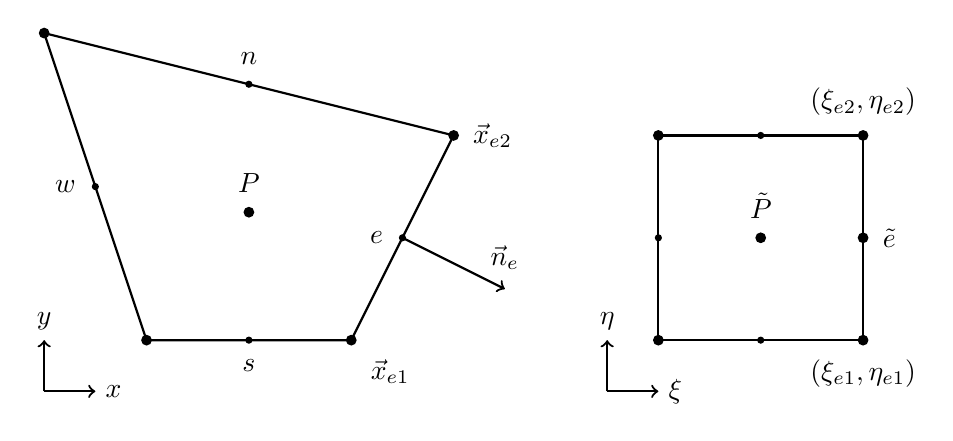
\begin{tikzpicture}[scale=1.3]
  \draw[->, thick] (-1,-0.5) -- (-0.5,-0.5) node[right] {$x$} coordinate(x axis);
  \draw[->, thick] (-1,-0.5) -- (-1,0) node[above] {$y$} coordinate(y axis);

  \draw[thick] (0,0) -- (2,0) -- (3,2) -- (-1, 3) --cycle;
  \fill (1,1.25) circle[radius=1.5pt];
  \node (x) at (1,1.25) [label=above:$P$] {};
  \fill (2,0) circle[radius=1.5pt];
  \node (x) at (2,0) [label=below right:$\vec x_{e1}$] {};
  \fill (3,2) circle[radius=1.5pt];
  \node (x) at (3,2) [label=right:$\vec x_{e2}$] {};

  \fill (-1,3) circle[radius=1.5pt];
  \fill (0,0) circle[radius=1.5pt];

  \fill (1,0) circle[radius=1pt];
  \node (x) at (1,0) [label=below:$s$] {};
  \fill (2.5,1) circle[radius=1pt];
  \node (x) at (2.5,1) [label=left:$e$] {};
  \fill (1,2.5) circle[radius=1pt];
  \node (x) at (1,2.5) [label=above:$n$] {};
  \fill (-0.5,1.5) circle[radius=1pt];
  \node (x) at (-0.5,1.5) [label=left:$w$] {};


  \draw[->, thick] (2.5,1) -> (3.5,0.5);
  \node (x) at (3.5,0.5) [label=above:$\vec n_e$] {};



  % xi-eta
  \draw[->, thick] (4.5,-0.5) -- (5,-0.5) node[right] {$\xi$} coordinate(x axis);
  \draw[->, thick] (4.5,-0.5) -- (4.5,0) node[above] {$\eta$} coordinate(y axis);

  \draw[thick] (5, 0) rectangle (7, 2);
  \fill (7, 1)  circle[radius=1.5pt];
  \node (x) at (7,1) [label={right}:{$\tilde{e}$}] {};

  \fill (5, 0)  circle[radius=1.5pt];
  \fill (5, 2)  circle[radius=1.5pt];
  \fill (5, 1)  circle[radius=1pt];
  \fill (6, 2)  circle[radius=1pt];
  \fill (6, 0)  circle[radius=1pt];

  \fill (7, 0)  circle[radius=1.5pt];
  \node (x) at (7,0) [label=below:{$(\xi_{e1},\eta_{e1})$}] {};
  \fill (7, 2)  circle[radius=1.5pt];
  \node (x) at (7,2) [label=above:{$(\xi_{e2}, \eta_{e2})$}] {};

  \fill (6, 1)  circle[radius=1.5pt];
  \node (x) at (6,1) [label=above:{$\tilde{P}$}] {};
\end{tikzpicture}
